% xv2-acmsmall-sample.tex, dated March 6 2012
% This is a sample file for ACM small trim journals
%
% Compilation using 'acmsmall.cls' - version 1.3 (March 2012), Aptara Inc.
% (c) 2010 Association for Computing Machinery (ACM)
%
% Questions/Suggestions/Feedback should be addressed to => "acmtexsupport@aptaracorp.com".
% Users can also go through the FAQs available on the journal's submission webpage.
%
% Steps to compile: latex, bibtex, latex latex
%
% For tracking purposes => this is v1.3 - March 2012

\documentclass[prodmode,acmtecs]{acmsmall} % Aptara syntax


% Package to generate and customize Algorithm as per ACM style
\usepackage[ruled]{algorithm2e}
\renewcommand{\algorithmcfname}{ALGORITHM}
\SetAlFnt{\small}
\SetAlCapFnt{\small}
\SetAlCapNameFnt{\small}
\SetAlCapHSkip{0pt}
\IncMargin{-\parindent}

% Metadata Information
% \acmVolume{9}
% \acmNumber{4}
% \acmArticle{39}
% \acmYear{2010}
% \acmMonth{3}

% Copyright
%\setcopyright{acmcopyright}
%\setcopyright{acmlicensed}
%\setcopyright{rightsretained}
%\setcopyright{usgov}
%\setcopyright{usgovmixed}
%\setcopyright{cagov}
%\setcopyright{cagovmixed}

% DOI
% \doi{0000001.0000001}

%ISSN
% \issn{1234-56789}

% Document starts
\begin{document}

% Page heads
\markboth{Y. Xie et al.}{Ranking Code Completion Candidates}

% Title portion
\title{Ranking Code Completion Candidates}
\author{Yanan Xie
\affil{yaxie@ucsc.edu}
Yifei Wu
\affil{ywu151@ucsc.edu}
Ziyi Chen
\affil{zchen139@ucsc.edu}
}

\begin{abstract}
Code completion is becoming a basic feature to all kinds of IDEs. It helps programmers to avoid typos and learn new languages fast. With the development of hardware performance and machine learning techniques, a lot of work could be done to further improve the code completion performance. Traditional code completion function lists all reserved words and variable names that match user’s input and then rank those matches in alphabetical order. We propose a new code completion candidate ranking method which aims at ranking those candidates with contextual syntax and semantic information. A code completion plugin is also built for Sublime Text - a very popular cross-platform code editor.
\end{abstract}


\maketitle


\section{Introduction}
\section{Related work}
\section{Ranking variables}
In this section, we talk about how to rank variables. According our experience, recently modified(assigned) or declared variables are more likely to be used. So we evaluate the relation of the distance between declaration/assignment and reference of variables, in order to rank previous variables at a certain point according to the distance. \\
We download git source code from github, which is written by c language, as our training data. Then we use Clang to generate AST of all those c files. Clang is a compiler front-end which is faster and neater that gcc. An example of ast is Fig. \ref{fig:ast example}. The front part is all "TypedefDecl", which is the ast structure of head file. But we only need to find out all declaration and assignment operation in cpp file. Since variables are only effective in certain function, we first find out all functions by "FunctionDecl" and then look out corresponding variables. The declaration statement is shown as "DeclStmt" as well as the function parameter "ParmVarDecl". The assignment statement consists of "BinaryOperator" with "=" and "UnaryOperator", which is "++" or "--". Use function name and variable name as key, ast line number and variable numbers as value to generate a dictionary. Then match all "DeclRefExpr" to find out usage of variables and use former dictionary to find distance of most recently declaration and modification. The result is shown below;

                                                           



\section{Modeling syntax}
In this part, we will try to figure out the relation between different types. At the beginning, we deal with the ast files we get from last part.\\
An example of ast is Fig. \ref{fig:ast example}.\\
The first token(ForStmt, DeclStmt, VarDel, IntegerLiteral) in each line is the type in ast. After learning the source codes of git, we get more than 70 kinds of different types. However, this project only aims on alphabet. In other words, we only deal with type-names, variable names, function names and reserved words. Thus, we should simplify these kinds of types. 
Here are our rules of simplification:\\
If a token contains “Decl”, we sort it to declaration, which is the format of “type-name + variable names”, \\
If a token contains “Expr”, we sort it to expression, which begins with “variable names”,\\
If a token contains “Stmt”, we remain it as reserved word, such as “ForStmt” is “for”, “WhileStmt” is “while”,\\
If a toke not contains “Decl”, “Expr”, “Stmt”, we sort it to else and ignore it in the following process.\\
After simplification, we get 22 kinds of types.\\
Then I calculate order-relations in all ast files. I calculate two kinds of relations. One is A$\longrightarrow$B. Another is A$\longrightarrow$B$\longrightarrow$C. Using these statistics results. We can get the possibility of all types when we know the previous code. \\
Table \ref{tab:SyntaxOne}. is part of statistics result of A$\longrightarrow$B and Table \ref{tab:SyntaxTwo}. is part of statistics result of A$\longrightarrow$B$\longrightarrow$C. From this we can see that with privous two tokens we can get a more accurate token.\\

\begin{figure}
\centerline{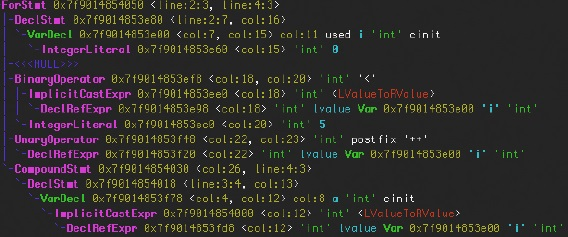
\includegraphics[width=0.9\textwidth]{ast_example.jpg}}
\caption{ast example}
\label{fig:ast example}
\end{figure}


\begin{table}%
\tbl{Partial Relation A$\longrightarrow$B\label{tab:SyntaxOne}}{%
\begin{tabular}{|l|l|l|l|}
\hline
Condition	 &Top Candidate	 &2nd Candidate	 &3rd Candidate\\\hline
FunctionDecl &	Declaration	 &FunctionDecl	 &ReturnStmt\\\hline
Declaration	 &Declaration &	FunctionDecl	 &Variable\\\hline
ReturnStmt	 &Variable	 &IfStmt	 &ForStmt\\\hline
Variable	 &Variable &	ReturnStmt	 &IfStmt\\\hline
IfStmt &	Variable	 &- &	-\\\hline
WhileStmt &	Variable &	-	 &-\\\hline
ForStmt	 &Declaration	 &Variable	 &IfStmt\\\hline
ContinueStmt	 &IfStmt	 &Variable	 &CaseStmt\\\hline
\end{tabular}}
\end{table}%


\begin{table}%
\tbl{Partial Relation A$\longrightarrow$B$\longrightarrow$C\label{tab:SyntaxTwo}}{%
\begin{tabular}{|l|l|l|l|}
\hline
Condition A&Condition B	 &Top Candidate	 &2nd Candidate\\\hline
empty &	FunctionDecl	 &Declaration	 &-\\\hline
FunctionDecl	 &Declaration &	Declaration	 &FunctionDecl\\\hline
Declaration	 &Declaration	 &Declaration	 &ForStmt\\\hline
Declaration	 &ReturnStmt &	Variable	 &-\\\hline
Declaration &	Variable	 &Variable &	-\\\hline
Declaration &	IfStmt &	Variable	 &-\\\hline
\end{tabular}}
\end{table}%




\section{Hacking the editor}



This is to show how to attach figure and table.

\begin{figure}
\centerline{
\includegraphics{acmsmall-mouse}}
\caption{Code before preprocessing.}
\label{fig:one}
\end{figure}

\begin{table}%
\tbl{Simulation Configuration\label{tab:one}}{%
\begin{tabular}{|l|l|}
\hline
TERRAIN{$^a$}   & (200m$\times$200m) Square\\\hline
Node Number     & 289\\\hline
Node Placement  & Uniform\\\hline
Application     & Many-to-Many/Gossip CBR Streams\\\hline
Payload Size    & 32 bytes\\\hline
Routing Layer   & GF\\\hline
MAC Layer       & CSMA/MMSN\\\hline
Radio Layer     & RADIO-ACCNOISE\\\hline
Radio Bandwidth & 250Kbps\\\hline
Radio Range     & 20m--45m\\\hline
\end{tabular}}
\begin{tabnote}%
\Note{Source:}{This is a table
sourcenote. This is a table sourcenote. This is a table
sourcenote.}
\vskip2pt
\Note{Note:}{This is a table footnote.}
\tabnoteentry{$^a$}{This is a table footnote. This is a
table footnote. This is a table footnote.}
\end{tabnote}%
\end{table}%

\section{Conclusions}

Just to show how to cite reference. \cite{Abril07},


% Acknowledgments
\begin{acks}
The authors would like to thank Dr. Maura Turolla of Telecom
Italia for providing specifications about the application scenario.
\end{acks}

% Bibliography
\bibliographystyle{ACM-Reference-Format-Journals}
\bibliography{acmsmall-sample-bibfile}
 


\end{document}
% End of v2-acmsmall-sample.tex (March 2012) - Gerry Murray, ACM


